\documentclass[../main.tex]{subfiles}

\begin{document}

\section{Elektrozwakke precisie testen}%
\label{sec:elektrozwakke_precisie_testen}

De eerste oplossing die aan bod is gekomen om de korte dracht van de zwakke wisselwerking te verklaren is de massa van het intermediaire boson.

\subsection{Zwakke uitwisselings deeltjes}%
\label{sub:zwakke_uitwisselings_deeltjes}

Zoals op het einde van vorig hoofdstuk is gezegd zijn de uitwisselings deeltjes van de zwakke interactie $W_1$, $W_2$ en $W_3$. De eerste 2 bosonen vormen samen de geladen zwakke stromen $W^\pm$. Hierbij was een voorspelling gedaan van de massa's van deze deeltjes enkele GeV te zijn. Wat is $W_3$ nu? Dit kan niet anders dan een neutraal deeltje zijn. Het eerste waar me dan aan denkt is het foton maar dit is niet mogelijk vanwege de koppeling met neutrinos. Er wordt gepostuleerd dat er ook een isospin singlet moet bestaan $B^0$ die ook neutraal is. Deze 2 kunnen opmengen tot $A^\mu$ en $Z^\mu$.
\begin{equation}
    \begin{aligned}
        \label{eq:zwakke_boson_opmenging}
        \begin{pmatrix}
            A^\mu\\
            Z^\mu
        \end{pmatrix}
        =
        \begin{pmatrix}
            \cos\theta_W & \sin\theta_W\\
            -\sin\theta_W & \cos\theta_W
        \end{pmatrix}
        \begin{pmatrix}
            B^0\\
            W^3
        \end{pmatrix}
    \end{aligned}
\end{equation}
$Z$ komt overeen met de zwakke wisselwerking en $A$ met de elektromagnetische. Wat een unificatie zal zijn tussen de zuivere zwakke bosonen en de elektrozwakke bosonen.

\subsection{Neutrale zwakke stroom}%
\label{sub:neutrale_zwakke_stroom}

De reden voor deze drang om een elektrozwakke unificatie te vinden stamt uit het vinden van de zuivere interactie stroom naast een axiale in de zwakke interactie experimenten (wat neerkomt op een zuivere vector stroom tussen specifieke chirale deeltjes). We hebben in deze 2 theorieën 2 uitwisselings deeltjes met gelijke kwantumgetallen die dan uiteraard zullen opmengen. De reden waarom de sterke wisselwerking niet bij wordt gehaald is omdat deze alleen met de quarks zal interageren en niet met de leptonen.\\
De elektrozwakke unificatie zegt ons dat er naast de geladen stromen ook een neutrale stroom zwakke stroom moet zijn  aan de hand van $Z^0$ uitwisseling. Het probleem is dat deze experimenteel nooit gezien worden. Deze zijn enkel zichtbaar als alle andere kanalen onderdrukt worden. Een mogelijke oplossing hiervoor is te werken met de neutrinos die alleen zwak kunnen interageren. In 1973 is in een bubbel experiment voor het eerst zo een neutrale stroom waargenomen en is dus aangetoond dat de neutrale stromen bestaan.

\subsection{Uitwisselings bosonen}%
\label{sub:uitwisselings_bosonen}

Nu we weten dat deze deeltjes bestaan willen we die natuurlijk ook effectief aanmaken. Om dit te doen hebben we ze in CERN de SPS-collider omgebouwd om $p\overline p$ verstrooiingen uit te voeren. De reden waarom we effectief $\overline p$ gebruiken is als we een antiquark uit $p$ moeten halen dat dit enkel een zeequark kan zijn en dus maar een kleine fractie van het proton zal hebben. Hierdoor is er niet genoeg energie om een $W$ boson aan te maken. Als je een $\overline p$ gebruikt zal het antiquark nu een veel grotere fractie van het proton hebben en we genoeg energie hebben om een $W$ boson aan te maken.
\begin{equation}
    \begin{aligned}
        \label{eq:w_productie}
        p + \overline p \rightarrow W + \text{rest} \rightarrow e\nu / \mu\nu + \text{rest}
    \end{aligned}
\end{equation}
Het maken van een anti protonenbundel is niet zo moeilijk. Schiet een protonenbundel op een target waar onderandere antiprotonen uit komen. Het probleem hierbij is dat deze alle richtingen uitgaan. Door een magneet in de buurt te zetten kan je deze colimeteren tot een bundel in een buis. Op dit moment divergeren de antiprotonen nog. Door deze af te koelen is het mogelijk om de antiprotonen allemaal in dezelfde richting te laten gaan. Door het heisenberg principe zal bij het samendrukken van de bundel in de ene richting deze in de andere richting uitzetten. De manier dat omzeilt kan worden is door causaliteit. Door he constant zijn van de lichtsnelheid is het mogelijk om in vogelvlucht informatie sneller aan de andere kant van de ring te krijgen en die informatie te gebruiken om de bundel bij te sturen.\\
Het probleem bij deze experimenten is dat de energie en momentum van de initiële quark en antiquark niet perfect geweten zijn. Het $W^+$ boson zal dus niet stil staan wat je niet kan meten. Wat we wel kunnen meten is de transversale impuls van het $W$ boson. Specifiek meten we $p_T(e)$ en omdat we met een hermetische detector werken is $p_T(\nu) = p_T(\text{missing}$. In de transversale richting is er geen boost en is $p_T$ dus Lorentz invariant. In het ruststelsel van $W$ is $|\vec{p}(e)|=-|\vec{p}(\nu)|$ en kunnen dus bepalen dat $p_T(e) = \frac{M_W}{2} \sin\theta^*$ met $\theta^*$ de de verval hoek in het ruststelsel.
\begin{equation}
    \begin{aligned}
        \label{eq:mom_dist}
        \frac{dn}{dp_T} &= \frac{dn}{d\theta^*} \frac{d\theta^*}{dp_T} \\
                        &= \frac{dn}{d\theta^*} \frac{1}{\sqrt{(M_W/2)^2-p^2}} 
    \end{aligned}
\end{equation}
Dit wil zeggen dat voor eender welke hoek afhankelijkheid er is in het aantal counts zullen we een piek waarnemen als $p_T=M_W/2$. Als we de transversale massa ($m_T=2p_T$) plotten in een histogram krijgen we dat de massa van het $W^+$ boson $M_W=80.0\pm 1.5$GeV is.

\begin{figure}[h]
    \centering
    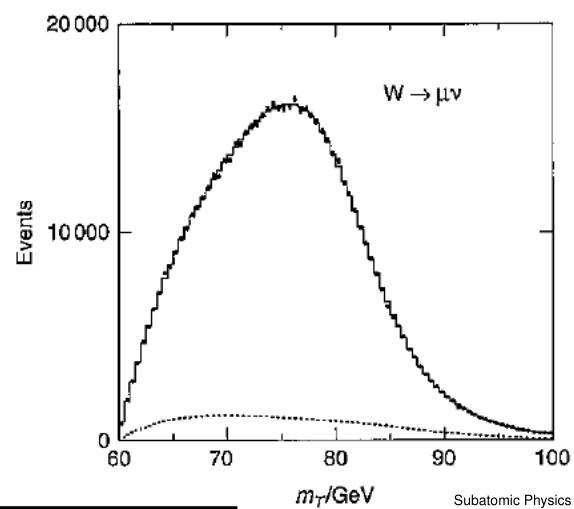
\includegraphics[width=0.3\linewidth]{elektroweak_precision_tests/w_boson_massa.png}
    \caption{Histogram van events in functie van de transversale massa}%
    \label{fig:elektroweak_precision_tests/w_boson_massa}
\end{figure}

Het meten van de massa van het $Z$ boson is een stuk makkelijker omdat we hier niet te maken hebben met een neutrino en de invariante massa rechtstreeks kunnen meten.
\begin{equation}
    \begin{aligned}
        \label{eq:z_productie}
        p + \overline p \rightarrow Z^0 + \text{rest} \rightarrow e^+/e^- (\mu^+/\mu^-) + \text{rest}
    \end{aligned}
\end{equation}
De massa van dit boson is $M_Z=91.5\pm 1.7$GeV.

\begin{figure}[h]
    \centering
    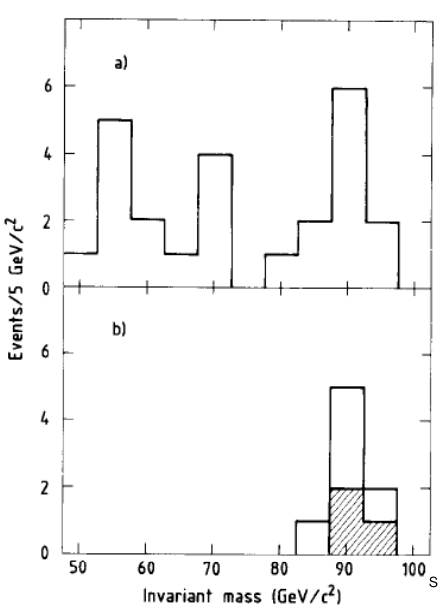
\includegraphics[width=0.3\linewidth]{elektroweak_precision_tests/z_boson_massa.png}
    \caption{Bepalen van de massa van het $Z$ boson}%
    \label{fig:elektroweak_precision_tests/z_boson_massa}
\end{figure}

\subsection{Spin van $W$}%
\label{sub:spin_van_w_}

\begin{figure}[h]
    \centering
    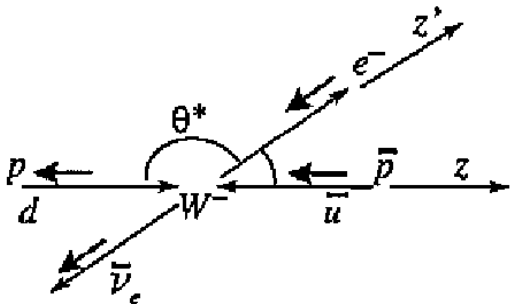
\includegraphics[width=0.4\linewidth]{elektroweak_precision_tests/spin_van_w.png}
    \caption{Schema van de kinematica van een verstrooiing om de spin van $W$ te bepalen}%
    \label{fig:elektroweak_precision_tests/spin_van_w}
\end{figure}

Nemen we aan dat de V-A theorie correct is en we laten een anti-up in een down quark annihileren tot een $W^-$ boson. V-A zegt dat $d$ een linkshandig deeltje moet zijn en zijn spin is dus antiparallel aan de bewegingsrichting. Voor $\overline u$ zegt V-A dat dit een rechtshandig deeltje is en ligt zijn spin parallel aan zijn bewegingsrichting. De spin van $W^-$ is de combinatie van de 2 spins, $J=1$ en $J_z=-1$. De $-1$ projectie op de z-richting is door conventie dat de z-richting gelijk wordt gesteld aan de proton richting. Vervolgens laten we $W^-$ vervallen naar $e^-$ en $\overline \nu$. Omdat we met een elektron te maken hebben weten we dat het intermediaire boson een $W^-$ boson zal zijn. Voor de uitgaande deeltjes kunnen we nu ook als een kwantisatieas zien met $e^-$ linkshandig en $\overline \nu$ rechtshandig. Dit geeft ons terug een projectie van de spin op deze as $J_{z'}=-1$. We moeten dus de waarschijnlijkheid bepalen waarbij $J_z=-1$ wordt omgezet in $J_{z'}=-1$. Dit gebeurt aan de hand van de rotatie matrices.
\begin{equation}
    \begin{aligned}
        \label{eq:kans_proj_omz}
        \frac{d\sigma}{d\Omega} &\propto (d_{-1,-1}^1)^2\\
                                &\propto \left[ \frac{1}{2} (1+\cos\theta^*)\right]^2
    \end{aligned}
\end{equation}
Kijken we nu experimenteel naar de hoekdistributie zien we duidelijk dat het $W^-$ een spin van 1 moet hebben.

\begin{figure}[h]
    \centering
    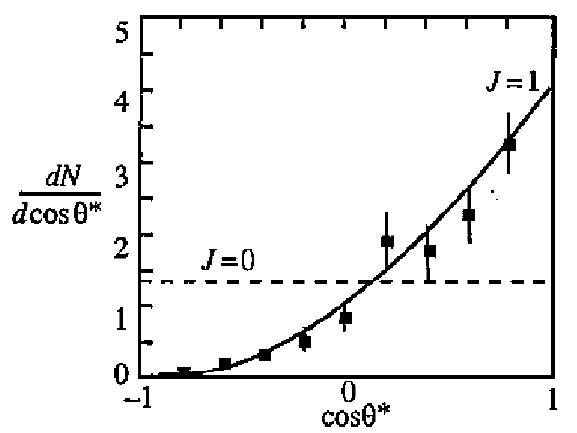
\includegraphics[width=0.4\linewidth]{elektroweak_precision_tests/spin_van_w_resultaten.png}
    \caption{Experimentele resultaten van de spin van $W$}%
    \label{fig:elektroweak_precision_tests/spin_van_w_resultaten}
\end{figure}

\subsection{Elektrozwakke unificatie}%
\label{sub:elektrozwakke_unificatie}

Kijken we nu terug naar de stromen van de geladen zwakke interactie.
\begin{equation}
    \begin{aligned}
        \label{eq:stroom_geladen_zwakke_int}
        \begin{matrix}
            W^\pm = \frac{1}{\sqrt{2}} (W^1\pm iW^2) & j^\pm = \frac{1}{\sqrt{2}} (j_1\pm ij_2) \\
            j_\mu^- = \overline\nu_{eL}\gamma_\mu e_L^- & j_\mu^+ = \overline e_L^-\gamma_\mu\nu_{eL}
        \end{matrix}
    \end{aligned}
\end{equation}
De zwakke interactie heeft 3 intermediaire bosonen, het 3de boson is een isocalaire interactie $B$. De $SU(2)$ groep kunnen we unificeren tot $SU(2)\otimes U(1)$. $U(1)$ is hier niet de elektromagnetische groep omdat $B$ niet exact het foton kan zijn. Voor die wisselwerking is de zwakke hyperlading toegevoegd $Y_W = 2(Q-I_z)$. Een aantal voorbeelden van de zwakke hyperlading zijn gegeven in tabel \ref{tab:zwakke_hyperlading}.

\begin{table}[h]
    \centering
    \caption{Voorbeelden van de hyperlading}
    \label{tab:zwakke_hyperlading}
    \begin{tabular}{cccc}
                & $Y_W$ &       & $Y_W$ \\
        \hline
        $\nu_L$ & -1    & $u_L$ & $\frac{1}{3}$\\
        $l_L^-$ & -1    & $d_L$ & $\frac{1}{3}$\\
                &       & $u_R$ & $\frac{4}{3}$\\
        $l_R^-$ & -2    & $d_R$ & $-\frac{2}{3}$\\

    \end{tabular}
\end{table}

Mengen we nu $W_3$ en $B$ op dan krijgen we 
\begin{equation}
    \begin{aligned}
        \label{eq:w_b_mixing}
        \begin{pmatrix}
            Z^0\\
            A
        \end{pmatrix}
        &= \frac{1}{\sqrt{g^2+g'^2}} 
        \begin{pmatrix}
            g & -g'\\
            g' & g
        \end{pmatrix}
        \begin{pmatrix}
            W_3\\
            B
        \end{pmatrix}\\
        &=
        \begin{pmatrix}
            \cos\theta_W & -\sin\theta_W\\
            \sin\theta_W & \cos\theta_W
        \end{pmatrix}
        \begin{pmatrix}
            W_3\\
            B
        \end{pmatrix}
    \end{aligned}
\end{equation}
met $g$ de zwakke koppelingsconstante en $g'$ de koppelingsconstante die we niet kennen waarmee $B$ aan de zwakke hyperlading koppelt. De weinberg hoek kan geschreven worden als: $\theta_W\equiv \tan^{-1} \frac{g'}{g}$. Nu wordt de Lagrangiaan gegeven door:
\begin{equation}
    \begin{aligned}
        \label{eq:elektozwakke_lagrangiaan}
        \mathcal{L} &= g(j_\mu^1W_1^\mu+j_\mu^2W_2^\mu+j_\mu^3W_3^\mu)+ \frac{g'}{2} j_\mu^YB^\mu\\
                    &= \frac{g}{\sqrt{2}} (j_\mu^-W_+^\mu+j_\mu^+W_-^\mu) + j_\mu^3(gW_3^\mu-g'B^\mu) + g'j_\mu^{EM}B^\mu\\
                    &= \frac{g}{\sqrt{2}} (j_\mu^-W_+^\mu+j_\mu^+W_-^\mu) + \frac{g}{\cos\theta_W} (j_\mu^3 - \sin^2\theta_Wj_\mu^{EM})Z^\mu + g\sin\theta_Wj_\mu^{EM}A^\mu
    \end{aligned}
\end{equation}
Hierbij kunnen we mooi zien in de eerste lijn dat de $W$'s interageren met een strekte $g$ en $B$ met een sterkte $g'$. Als we ervan uit gaan dat $A$ een foton beschrijft moet $g\sin\theta_W \propto e$ zijn of exact $g\sin\theta_W = \sqrt{4\pi\alpha}$. We zien dus eigenlijk dat g zo  goed als gelijk is aan de elektromagnetische koppeling. Uit de 2de term krijgen we de koppelingsterkte van het $Z$ boson.
\begin{equation}
    \begin{aligned}
        \label{eq:koppeling_z}
        g_Z &= \frac{g}{\cos\theta_W} (I_z - Q\sin^2\theta_W)\\
            &= \frac{g}{\cos\theta_W} c_Z\\
            c_Z = I_z - Q\sin^2\theta_W
    \end{aligned}
\end{equation}
Hier is $c_Z$ equivalent met de kleurfactoren van QCD. Ten laatste voor de $W$ koppeling moet deze $g$ overeen komen met de propagator term uit de klassieke theorie
\begin{equation}
    \begin{aligned}
        \label{eq:koppeling_w}
        G_F = \frac{\sqrt{2}g^2}{8M_W^2} 
    \end{aligned}
\end{equation}
In de propagator term komt de massa van het $W$ boson voor:
\begin{equation}
    \begin{aligned}
        \label{eq:massa_w}
        M_W &= \frac{g^2\sqrt{2}}{8G_F} \\
            &= \sqrt{ \frac{\pi\alpha}{\sqrt{2}G_F}} \frac{1}{\sin\theta_W} = \frac{37.3}{\sin\theta_W} \text{GeV}
    \end{aligned}
\end{equation}
Zo is het mogelijk om de elektromagnetische en zwakke wisselwerking op te beschrijven in termen van 2 constantes: $\alpha$ en $\theta_W$.

\subsection{Massa van het $Z^0$-boson}%
\label{sub:massa_van_het_z_0_boson}

Gaan we ervan uit dat de massa van het $Z$ boson komt van het matrix element dan is $M_\phi^2 = \left<\phi|H|\phi\right>^2$. Zo krijgen we 3 vergelijkingen waarbij we gebruikt hebben dat het foton massaloos is en het foton en $Z$ boson orthogonaal zijn.
\begin{equation}
    \begin{aligned}
        \label{eq:massa_z}
        M_Z^2 &= M_W^2 \cos^2\theta_W + M_B^2\sin^2\theta_W - 2M_{BW}^2\cos\theta_W\sin\theta_W\\
        0=M_\gamma^2 &= M_W^2 \sin^2\theta_W + M_B^2\cos^2\theta_W + 2M_{BW}^2\cos\theta_W\sin\theta_W\\
        0=M_{Z\gamma}^2 &= (M_W^2-M_B^2) \sin\theta_W\cos\theta_W + M_{BW}^2(\cos^2\theta_W-\sin^2\theta_W)\\
                        &\Rightarrow M_Z = \frac{M_W}{\cos\theta_W}
    \end{aligned}
\end{equation}
Aan de hand van deze relatie tussen de massa van de $W$ en $Z$ bosonen is het mogelijk om de theorie te testen.

\subsection{Koppeling van het $Z^0$ boson}%
\label{sub:koppeling_van_het_z_0_boson}

Als we kijken naar de koppelingsconstante van het $Z$ boson zijn we geïnteresseerd in 1 specifieke term in de lagrangiaan.
\begin{equation}
    \begin{aligned}
        \label{eq:z_term_lagrangiaan}
        \frac{g}{\cos\theta_W} (j_\mu^3 - \sin^2\theta_Wj_\mu^\text{EM})Z^\mu
    \end{aligned}
\end{equation}
De koppelingsconstante voor links en rechtshandige deeltjes zal verschillen.
\begin{equation}
    \begin{aligned}
        \label{eq:z_koppelingsterkte}
        g_L &= I_z - Q\sin^2\theta_W\\
        g_R &= -Q\sin^2\theta_W
    \end{aligned}
\end{equation}
Hierbij komt de $I_z$ component van de $j^3$ stroom en de $Q\sin^2\theta_W$ component van de $j^\text{EM}$ stroom. Het is natuurlijk logisch dat de $I_z$ component 0 is voor de rechts chirale deeltjes omdat deze niet koppelen aan elkaar. Kijken we nu naar de zwakke koppelingsterkte in functie van de vector en axiale termen:
\begin{equation}
    \begin{aligned}
        \label{eq:zwakke_koppelingsconstante}
        c_V &= g_L + g_R = I_z - 2Q\sin^2\theta_W\\
        c_A &= g_L - g_R = I_z
    \end{aligned}
\end{equation}
Hier is het mogelijk om uit de polarisatie de links en rechts chirale koppeling component halen en die gebruiken om de $\theta_W$ te bepalen. Zo zien we voor verschillende deeltjes (tabel \ref{tab:v_a_comp_kc}) dat $c_A$ altijd $\pm1/2$ is en dat $c_V$ zal afhangen van de Weinberg hoek en de lading van het deeltje dat met $Z$ interageert. Er is dus geen universele koppelingsconstante.

\begin{table}[h]
    \centering
    \caption{vector en axiale componenten van de koppelingsconstante}
    \label{tab:v_a_comp_kc}
    \begin{tabular}{ccc}
                & $2c_V$                            & $2c_A$    \\
        $\nu$   & $+1$                              & $+1$      \\
        $e$     & $-1+4\sin^2\theta_W$              & $-1$      \\
        $u$     & $+1-\frac{8}{3}\sin^2\theta_W$    & $+1$      \\
        $d$     & $-1+\frac{4}{3}\sin^2\theta_W$    & $-1$      \\
    \end{tabular}
\end{table}

\subsection{$e^+e^-$ annihilatie}%
\label{sub:_e_e_annihilatie}

\begin{minipage}[c]{0.5\textwidth}
    \begin{center}
        \feynmandiagram[inline=(a), horizontal=a to b]{
            a -- [photon, edge label=\(\gamma\)] b,
            i1 [particle=\(e^-\)] -- [fermion] a,
            a -- [fermion] i2 [particle=\(e^+\)],
            fs 1 [particle=\(\overline f\)] -- [fermion] b,
            b -- [fermion] f2 [particle=\(f\)],
        };
    \end{center}
\end{minipage}\noindent
\begin{minipage}[c]{0.5\textwidth}
    \begin{center}
        \feynmandiagram[inline=(a), horizontal=a to b]{
            a -- [boson, edge label=\(Z\)] b,
            i1 [particle=\(e^-\)] -- [fermion] a,
            a -- [fermion] i2 [particle=\(e^+\)],
            f1 [particle=\(\overline f\)] -- [fermion] b,
            b -- [fermion] f2 [particle=\(f\)],
        };
    \end{center}
\end{minipage}
Hierbij zal er naast de elektromagnetische wisselwerking met een foton ook een mogelijkheid zijn om zwak te binden aan een $Z^0$ boson. Het is dus mogelijk om eender welk diagram met $\gamma$ een equivalent te tekenenen met een $Z^0$ boson. Uit deze diagrammen kunnen we nu 2 verschillende ladingen halen:
\begin{equation}
    \begin{aligned}
        \label{eq:e+_e-_lading}
        \begin{matrix}
            -i\frac{g^{\mu\nu}}{q^2} &&&& \frac{-ig^{\mu\nu}- \frac{q^\mu q^\nu}{M_Z^2} }{q^2-M_Z^2}
        \end{matrix}
    \end{aligned}
\end{equation}
Uit de 2de lading kunnen we zien dat deze zal divergeren als $q=M_Z^2$ wat we kunnen zien in experimenten.

\begin{figure}[h]
    \centering
    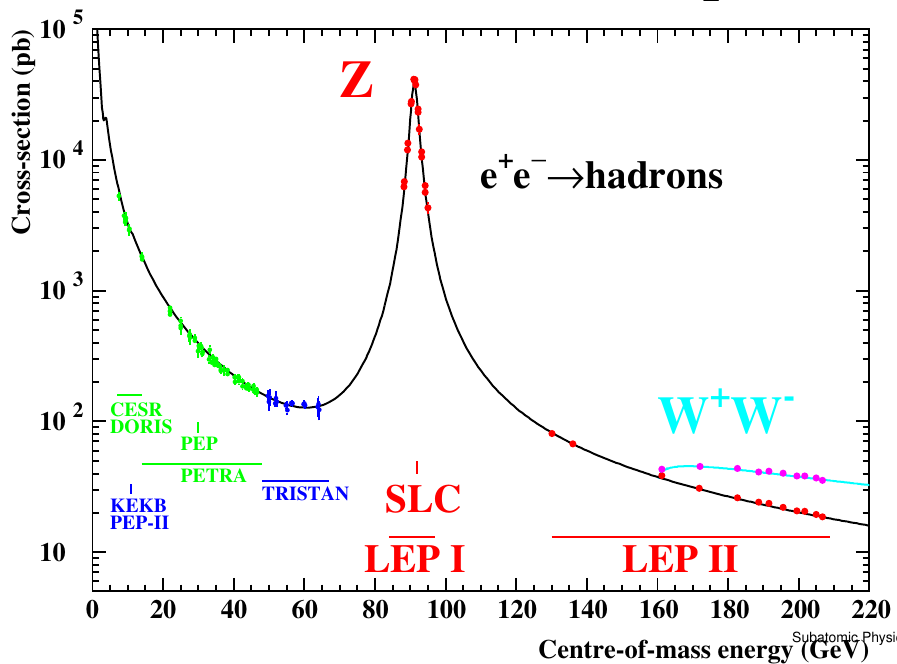
\includegraphics[width=0.6\linewidth]{elektroweak_precision_tests/e+e-_annihilatie.png}
    \caption{Resultaten naar het onderzoek van $e^+e^-$ annihilatie}%
    \label{fig:elektroweak_precision_tests/e+e-_annihilatie}
\end{figure}

\subsection{Het $Z$ boson}%
\label{sub:het_z_boson}

Brengen we alle werkzame doorsnedes van de mogelijke verval modes van het $Z$ boson samen tot een totale werkzame doorsnede.
\begin{equation}
    \begin{aligned}
        \label{eq:z_werkzame_doorsnede}
        \sigma_Z^0 = {\color{red} \frac{12\pi}{M_Z^2}} {\color{blue} \frac{\Gamma_e}{\Gamma_Z}} {\color{green} \frac{\Gamma_f}{\Gamma_Z}} \frac{s\Gamma_Z^2}{(s-M_Z^2)^2 + s^2\Gamma_Z^2/M_Z^2}
    \end{aligned}
\end{equation}
In het rood hebben we de propagator, in blauw de waarschijnlijkheid om een elektron te koppelen aan een $Z$ boson, in groen de waarschijnlijkheid om het $Z$ boson te koppelen aan een fermion en in het zwart de breit wigner term. Hierbij is $\Gamma_f$ de accumulatie van alle maniereb dat $Z$ naar quark-antisuark paren met uitzondering van $t\overline t$. De 0 in de exponent is om erop te duiden dat dit de nulde orde term is en dus de eenvoudigste benadering is. Uit de experimenten (figuur \ref{fig:elektroweak_precision_tests/het_z_boson}) kan je snel zien dat deze benadering nog verder uitgewerkt moet worden. Hier kan je een QED gecorrigeerde curve naast de gemeten curve zien. Dit is niets anders dan het in acht nemen dat één van de inkomende of uitgaande deeltjes een hoog energetisch foton uitstraalt of dat er een vertex correctie (inkomende of uitgaande deeltjes interageren met elkaar aan de hand van een foton) op de inkomende of uitgaande deeltjes krijgen. Deze geven dus een eerste orde correctie op $\sigma_Z^0$ die vrij belangrijk is omdat hoog energetische deeltjes, zeker elektronen, graag fotonen afstralen. In het geval dat er een zwaar quark-antiquark paar wordt aangemaakt zoals $b\overline b$ zal het veel onwaarschijnlijker zijn dat deze een foton zullen uitstralen.

\begin{figure}[h]
    \centering
    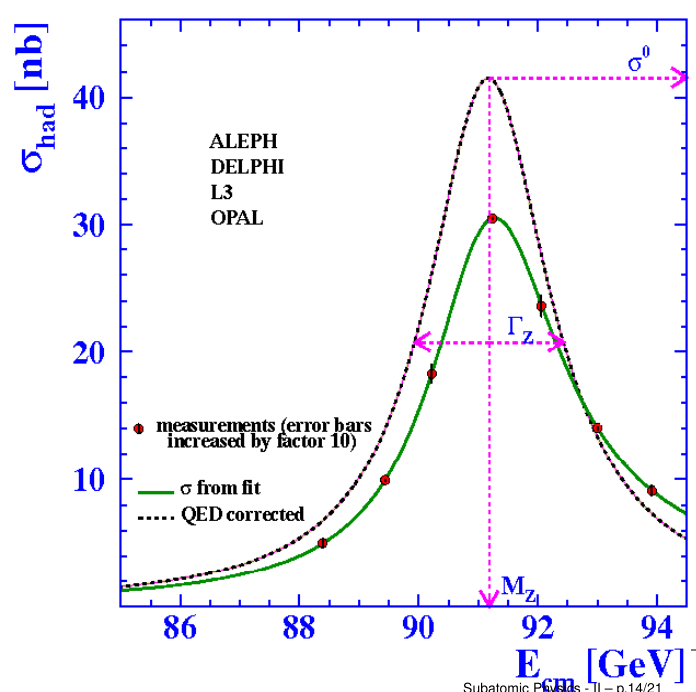
\includegraphics[width=0.6\linewidth]{elektroweak_precision_tests/het_z_boson.png}
    \caption{Experimentele waarden voor de cross sectie van $Z$ productie}%
    \label{fig:elektroweak_precision_tests/het_z_boson}
\end{figure}

Uit de gecorrigeerde metingen kunnen een aantal mooie gegevens gehaald worden. Eén hiervan is de breedte van het $Z$ boson wat de totale koppeling van het $Z$ boson zal geven aan alle mogelijke verval kanalen. De werkzame doorsnede voor $Z$ naar neutrino-antineutrino is onmeetbaar. We hebben daar gewoon de detectoren niet voor. Dit kan er uiteindelijk wel uit gehaald worden omdat we de totale breedte van $Z$ kennen en de partiële breedtes kunnen bepalen is het mogelijk om zo de breedte van $\nu\overline \nu$ te bepalen. Hiernaast kan uit al die metingen van de partiële breedtes terug de koppelingsconstantes bepaalt worden, $\Gamma_f \propto g_{v_f}^2+g_{A_f}^2$. Uit dit experiment kunnen we terug de massa en breedte van $Z$ bepalen. Deze zijn $M_Z = 91.1875 \pm 0.0021$GeV en $\Gamma_Z = 2.4952 \pm 0.0023$GeV. Uit de totale verval breedte kunnen we zien dat er 3 lichte neutrinos zijn, $n_\nu = 2.9840 \pm 0.0082$.

\subsection{Voorwaards-achterwaardse asymmetrie}%
\label{sub:voorwaards_achterwaardse_asymmetrie}

Uit zowel de Massa $Z$ en $W$ of de breedte van $Z$ is het mogelijk om de $\theta_W$ te bepalen. Er zijn nog vele andere manieren om dit te doen. Eén hiervan is de uit de Voorwaards-achterwaardse asymmetrie.\\
\begin{minipage}[c]{0.5\textwidth}
    \begin{center}
        \feynmandiagram[inline=(a), horizontal=a to b]{
            a -- [photon, edge label=\(\gamma\)] b,
            i1 [particle=\(e^-\)] -- [fermion] a,
            a -- [fermion] i2 [particle=\(e^+\)],
            fs 1 [particle=\(\overline f\)] -- [fermion] b,
            b -- [fermion] f2 [particle=\(f\)],
        };
    \end{center}
\end{minipage}\noindent
\begin{minipage}[c]{0.5\textwidth}
    \begin{center}
        \feynmandiagram[inline=(a), horizontal=a to b]{
            a -- [boson, edge label=\(Z\)] b,
            i1 [particle=\(e^-\)] -- [fermion] a,
            a -- [fermion] i2 [particle=\(e^+\)],
            f1 [particle=\(\overline f\)] -- [fermion] b,
            b -- [fermion] f2 [particle=\(f\)],
        };
    \end{center}
\end{minipage}
$e^+e^-\rightarrow f\overline f$ via de elektromagnetische wisselwerking is een pariteit behoudende term hebben m.a.w. is deze symmetrisch over een hoek van $90^\circ$. Daarentegen is een deel van $e^+e^-\rightarrow f\overline f$ via het $Z$ boson via de zwakke wisselwerking en zal de pariteit schenden. Deze zal wel doorgaan onder zowel $0^\circ$ als $180^\circ$ maar zal een assymetrie ondervinden die met het uitwisselen van een foton er niet zou zijn. Deze asymmetrie kan uitgeschreven worden in een cross sectie.
\begin{equation}
    \begin{aligned}
        \label{eq:fb_assym}
        \frac{d\sigma(s)}{d\cos\theta} = \sigma(s) \left[ \frac{3}{8} (1+\cos^2\theta + A_{FB}(s) \cos\theta) \right]
    \end{aligned}
\end{equation}
Hierbij is de laatste term te weiden aan het schenden van de pariteit. Deze forward-backward factor is niets anders dan $A_{FB} = \frac{N_F-N_B}{N_F+N_B}$. Waarbij de teller en noemer overeen komen met het experiment bij $0^\circ$ of $180^\circ$. In figuur \ref{fig:elektroweak_precision_tests/fb_assym} wordt de assymetrie uit gezet in functie van de $\cos(\theta)$. Hierbij is het heel duidelijk dat deze asymmetrisch zijn behalve in de piek waar het heel mooi symmetrisch is. De reden waarom het rond de piek zo goed als symmetrisch is, is omdat de assymetrie term afhangt van de interferentie tussen $\gamma$ en $Z$. Bij de piek is er nauwelijks nog $\gamma$ zijn en wordt de assymetrie heel klein.

\begin{figure}[h]
    \centering
    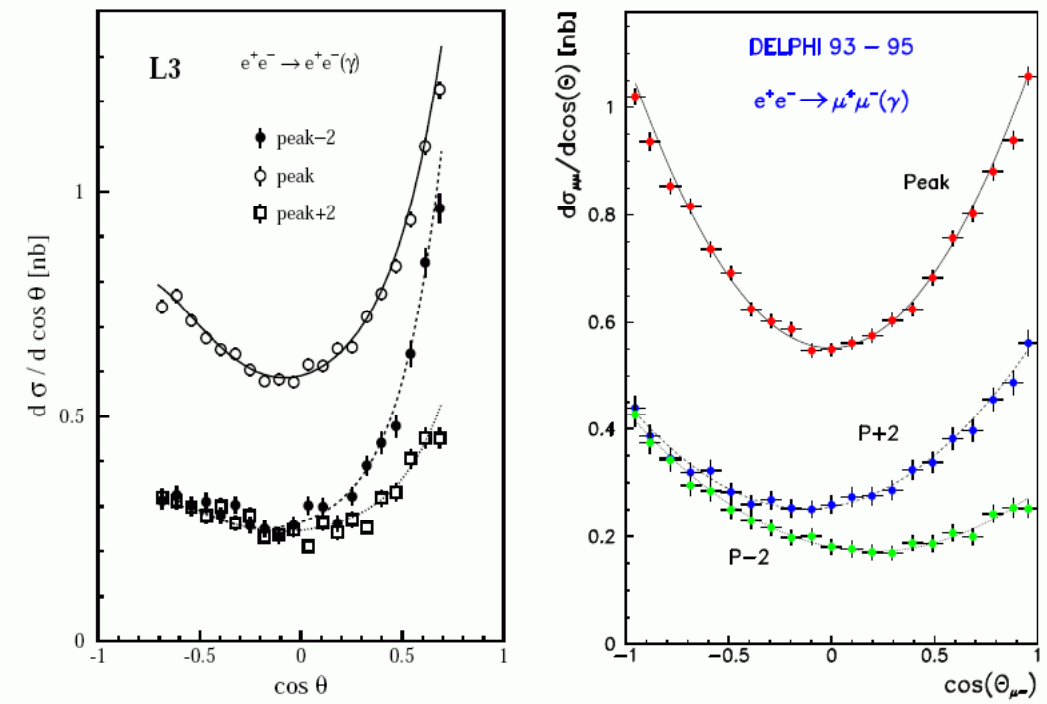
\includegraphics[width=0.4\linewidth]{elektroweak_precision_tests/fb_assym.png}
    \caption{Forward backward assymetrie experimenten.}%
    \label{fig:elektroweak_precision_tests/fb_assym}
\end{figure}

Uit de metingen van figuur \ref{fig:elektroweak_precision_tests/fb_assym} is het mogelijk om de de asymmetrie term in functie van de centre of mass energie te bepalen. Hierbij zijn de metingen terug gecorrigeerd voor de QED effecten die in eerste orde kunnen optreden. Deze is gevoelig voor de pariteit schending en dus voor de zwakke wisselwerking die gevoelig is voor $\theta_W$.

\begin{figure}[h]
    \centering
    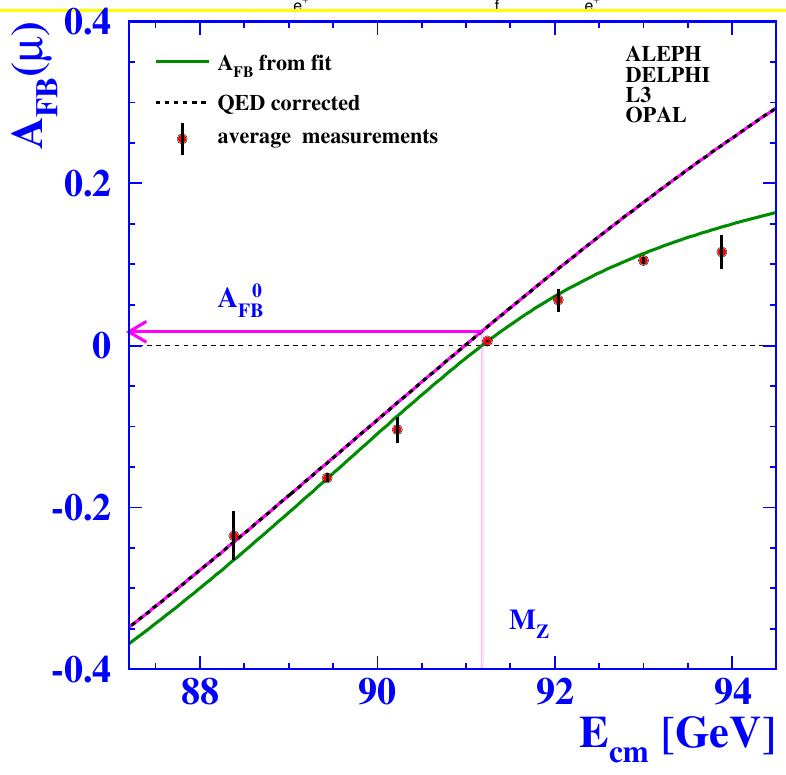
\includegraphics[width=0.5\linewidth]{elektroweak_precision_tests/fb_term.png}
    \caption{Asymmetrie term uit experimenten}%
    \label{fig:elektroweak_precision_tests/fb_term}
\end{figure}

\subsection{$Z$-koppeling}%
\label{sub:_z_koppeling}

Het visualiseren van de resultaten van de $Z$ koppeling zijn op verschillende manieren mogelijk. Om dit aan te tonen kijken we naar figuur \ref{fig:elektroweak_precision_tests/z_g_afhank} waar de koppeling van $Z$ aan de fermionen wordt weergeven in termen van vector en axiale koppeling. Hier kunnen we bijvoorbeeld zien dat $ee\rightarrow\mu\mu$ sterk gevoelig is voor de axiale component en veel minder gevoelig voor de vector component. Uit de resultaten uit 1987 kan ook gehaald worden dat $g_A \approx -0.5$ is en $g_V\approx 0$. Na vele jaren meten in het LEP is het mogelijk om een veel betere voorspelling te maken van $g_{Al} = -0.50123\pm0.00026$ en $g_V=-0.03783\pm0.00041$. Hieruit is het mogelijk om de Weinberg hoek heel precisie te bepalen.
\begin{equation}
    \begin{aligned}
        \label{eq:weinberg_hoek}
        \sin^2\theta_W = \frac{1}{4} \left( 1 - \frac{g_{Vl}}{g_{Al}} \right) = 0.23153 \pm 0.00016
    \end{aligned}
\end{equation}

\begin{figure}[h]
    \centering
    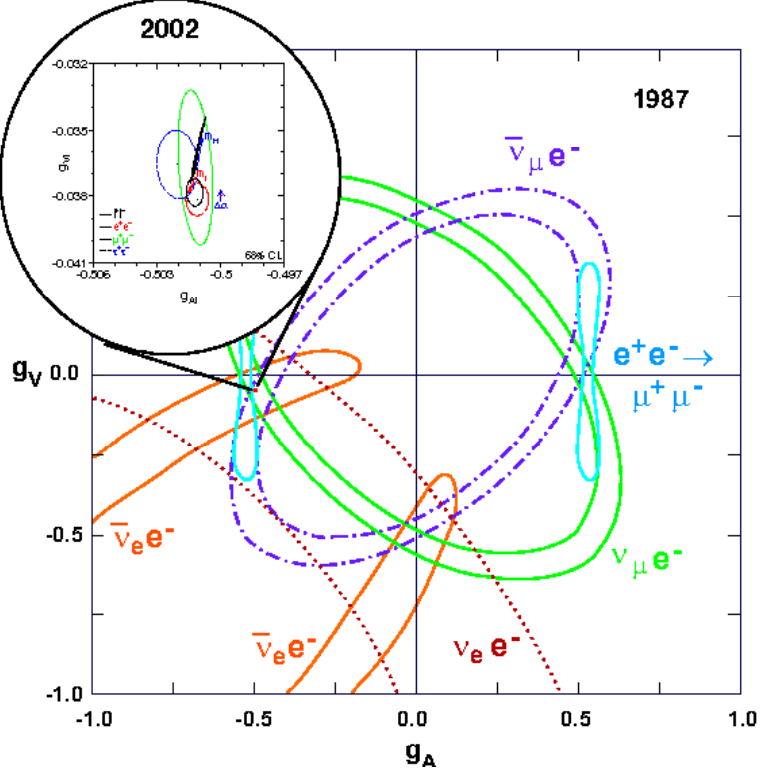
\includegraphics[width=0.4\linewidth]{elektroweak_precision_tests/z_g_afhank.png}
    \caption{Relatie tussen $g_V$ en $g_A$ voor het $Z$ boson}%
    \label{fig:elektroweak_precision_tests/z_g_afhank}
\end{figure}

\subsection{Het $W$ boson}%
\label{sub:het_w_boson}

De volgende stap in dit onderzoek was om $\theta_W$ te bepalen uit de relatie tussen de massa van $Z$ en $W$. In de 2de fase van LEP zijn de energieën opgedreven tot over 2 keer de massa van het $W$ boson, $\sqrt{s} > 2M_W$. Hierdoor is het mogelijk om  $W^+W^-$ te gaan creëren. Zo zijn er nieuwe diagrammen mogelijk.

\begin{figure}[h]
    \centering
    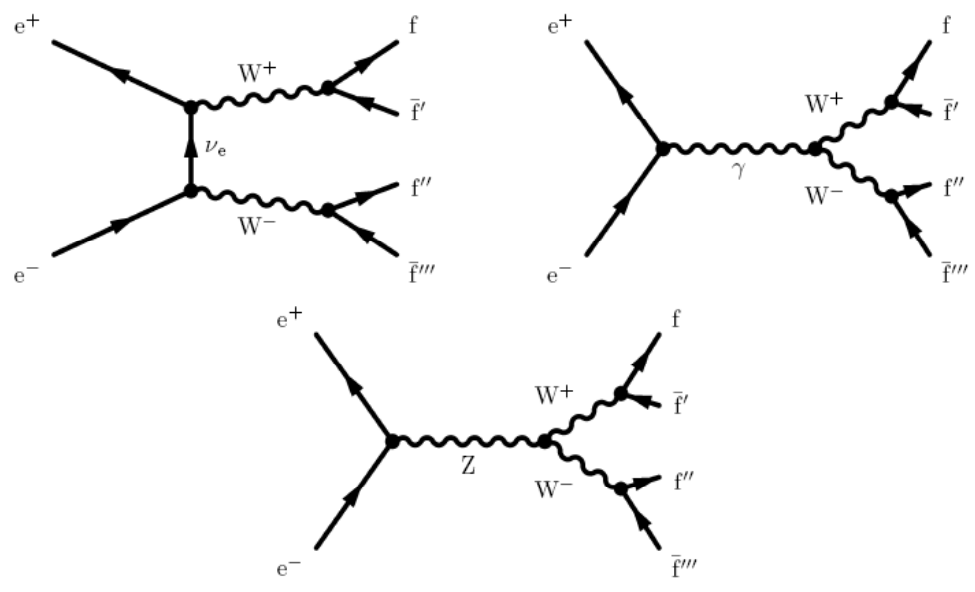
\includegraphics[width=0.6\linewidth]{elektroweak_precision_tests/reele_w_diagrammen.png}
    \caption{Feynman diagrammen voor reele $W^\pm$}%
    \label{fig:elektroweak_precision_tests/reele_w_diagrammen}
\end{figure}

Het laatste diagram hier gegeven is een typisch voorbeeld van een niet abelse groep te zijn waar de uitwisselingsbosonen met elkaar kunnen interageren. In dit geval $W_3$ met $W_{1/2}$. Deze $W$ bosonen kunnen op een aantal verschillende manieren vervallen.
\begin{equation}
    \begin{aligned}
        \label{eq:verval_w_boson}
        e^+e^- \rightarrow W^+W^- &\rightarrow q\overline q l\nu\\
                                  &\rightarrow l^+\nu l^-\overline \nu\\
                                  &\rightarrow q\overline q q\overline q
    \end{aligned}
\end{equation}
In het eerste geval hebben we 2 jets met een lepton en een neutrino, in het 2de geval enkel leptonen en neutrinos en in het 3de geval 4 jets. Het zal moeilijk zijn om verder te werken met de 2de verval optie omdat deze 2 niet te meten deeltjes bevatten. Om met de andere 2 onderzoek te doen reconstrueer je uit de impulsen van de uitkomende deeltjes de originele $W$ bosonen om uiteindelijk de invariante massa van het W boson te bekomen. Dit is mooi waargenomen in L3. In het rood zie je de monte carlo simulaties en in het zwart de metingen die gedaan zijn.

\begin{figure}[h]
    \centering
    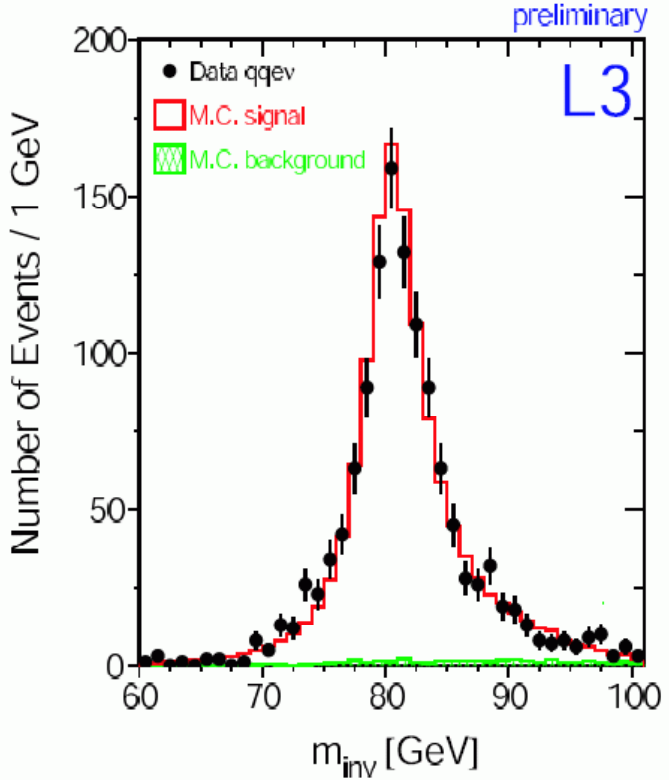
\includegraphics[width=0.4\linewidth]{elektroweak_precision_tests/invar_massa_w.png}
    \caption{L3 experiment om de massa van het $W$ boson te bepalen}%
    \label{fig:elektroweak_precision_tests/invar_massa_w}
\end{figure}

Uit deze metingen krijgen we $M_W = 80.412 \pm 0.042$GeV en $\Gamma_W = 2.150 \pm 0.091$GeV.

\subsection{Triple gauge koppeling}%
\label{sub:triple_gauge_koppeling}

\begin{figure}[h]
    \centering
    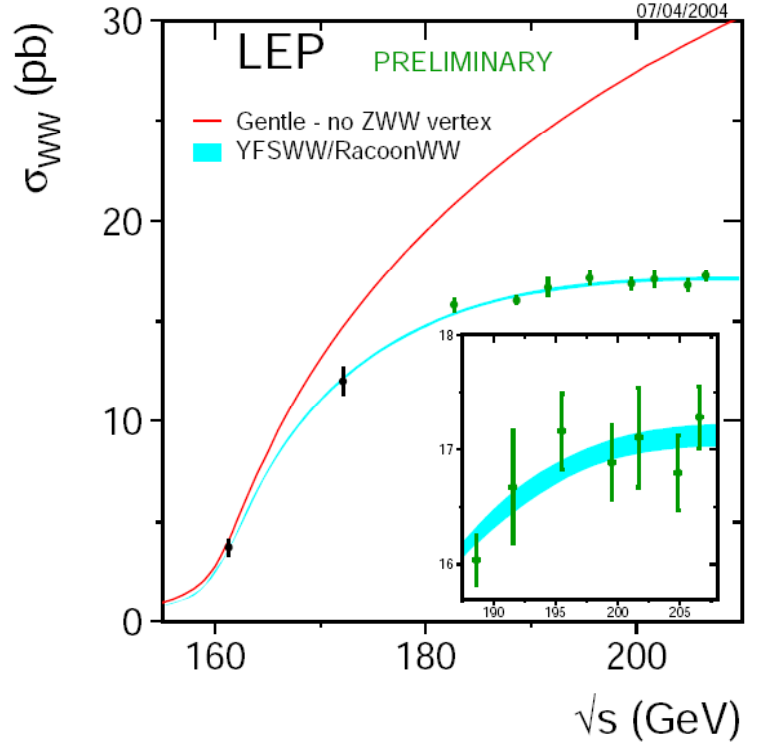
\includegraphics[width=0.4\linewidth]{elektroweak_precision_tests/w_sigma_sat.png}
    \caption{Cross sectie van triple gauge koppeling}%
    \label{fig:elektroweak_precision_tests/w_sigma_sat}
\end{figure}

Indien we de cross sectie voor de diagrammen in figuur \ref{fig:elektroweak_precision_tests/reele_w_diagrammen} berekenen, zien we niet fysische fenomenen. Voor het eerste diagram (CC(=charged-charged)-diagram) zien we dat $\sigma$ divergeert voor het tweede diagram (triple gauge koppeling met foton) is een deel van de divergentie van $\sigma$ verholpen maar zal deze uiteindelijk nog steeds divergeren. Het niet abelse karakter van het 3de diagram is nodig om $\sigma$ te laten convergeren en dat deze satureert tot een bepaalde waarde. In figuur \ref{fig:elektroweak_precision_tests/w_sigma_sat} staat in het rood de cross sectie indien de triple gauge koppeling $ZWW$ niet bestond. Het is duidelijk dat deze divergeert naar oneindig. Voeren we nu deze triple gauge koppeling toe zien we dat $\sigma$ zal afvlakken in het blauw en dat de experimenten in het groen deze mooi volgen. Dit bewijst dat we voor de zwakke wisselwerking te maken hebben met een niet abelse theorie.

\subsection{Standaard model radiatieve correcties}%
\label{sub:sm_radiatieve_correcties}

Bij het vergelijken van $\sin^2\theta_W$ gevonden uit het massaverschil van $Z$ en $W$ en de koppelingsterkte verschil van Z aan de vector en axiale component zien we een grote afwijking.
\begin{equation}
    \begin{aligned}
        \label{eq:vergelijken_weignberg_res}
        \sin^2\theta_W = \frac{1}{4}  \left( 1 - \frac{g_{Vl}}{g_{Al}} \right) &= 0.23153 \pm 0.00016\\
        \sin^2\theta_W = 1 - \frac{M_W^2}{M_Z^2} &= 0.22262 \pm 0.00045\\
        \approx 20\sigma \text{ deviatie}
    \end{aligned}
\end{equation}
Deze tonen aan dat onze theorie nog niet helemaal correct is. Bij het herbekijken van de koppelingstrektes zien we dat $g_{Al} = -0.50123 \pm 0.00026 \neq -\frac{1}{2}$ is. Bij het berekenen van $g_{Al}$ was verondersteld dat de $W$ en $Z$ bosonen massaloos zijn. Hoe deze bosonen massa krijgen hebben we nog niet besproken. Dit zal komen uit hogere orde termen. Omdat de zwakke interactie niet abels is zal deze naast het maken van fermionlussen ook interageren met zichzelf en het Higgs boson. Het zal het binden aan het Higgs boson zijn dat nu juist massa geeft aan de $W$ en $Z$ bosonen. Naast de correcties die moeten gemaakt worden voor de massa van de bosonen, $\propto \ln \frac{m_H}{M_W}$, is het bijvoorbeeld ook mogelijk dat $Z$ een $t\overline t$ lus maakt waarvoor men moet corrigeren proportioneel tot $M_t^2$. De koppelingen van het $Z$ boson zullen dus effectieve koppelingen worden die vrij gevoelig zijn voor de massa van de top quark en minder maar nog steeds gevoelig is voor de massa van het Higgs boson.

\begin{figure}[h]
    \centering
    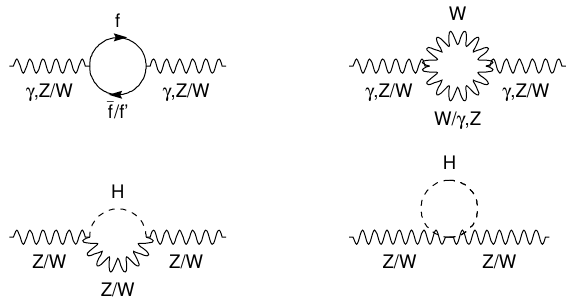
\includegraphics[width=0.6\linewidth]{elektroweak_precision_tests/hogere_orde_w.png}
    \caption{Hogere orde correctie termen}%
    \label{fig:elektroweak_precision_tests/hogere_orde_w}
\end{figure}

Deze correcties die we moeten doorvoeren zullen ons dus iets zeggen over de nog onbekende deeltjes $t$ en $H$. Laten we de theorie los op de experimentele resultaten kunnen we een voorspelling maken wat de massa van deze deeltjes zouden zijn. De massa van $t$ zal dus rond de $170-180$GeV moeten liggen. Indien dit niet zo zou zijn moeten de resultaten van het experiment meer verschoven worden naar rechtsboven. We zien ook dat de massa van het Higgs boson niet groot mag zijn omdat we anders ook terug te veel afwijken van de experimentele resultaten.

\begin{figure}[h]
    \centering
    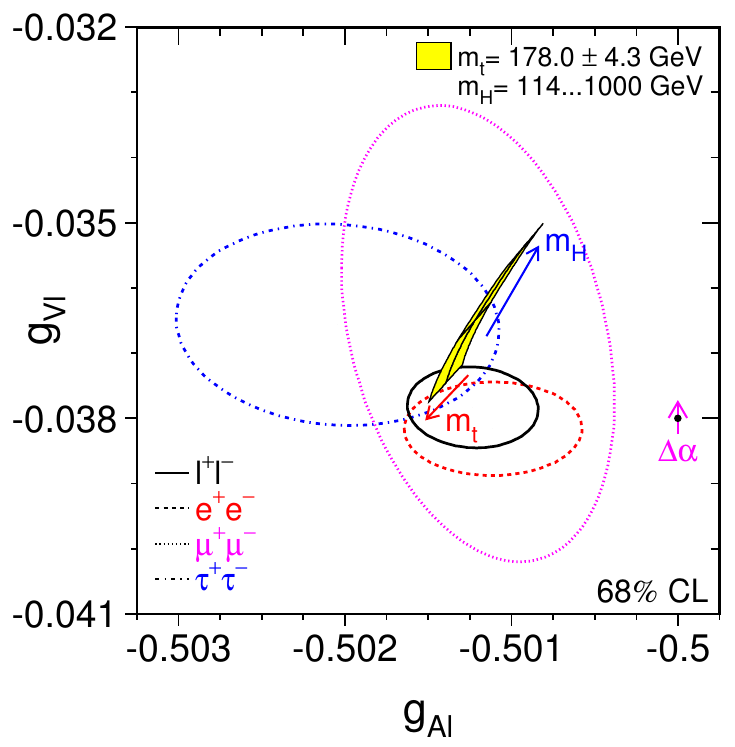
\includegraphics[width=0.4\linewidth]{elektroweak_precision_tests/massa_t_h_voorspellen.png}
    \caption{Voorspellingen van de massa's van $t$ en $H$}%
    \label{fig:elektroweak_precision_tests/massa_t_h_voorspellen}
\end{figure}

\subsection{De top quark}%
\label{sub:de_top_quark}

\begin{figure}[h]
    \centering
    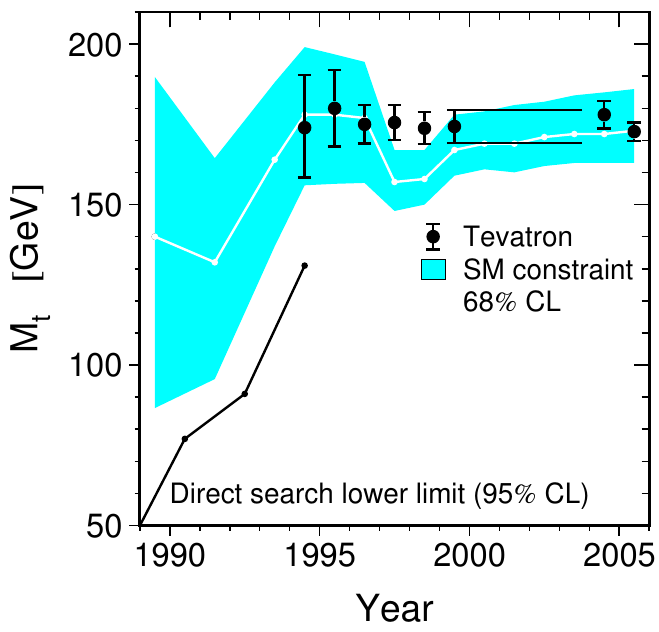
\includegraphics[width=0.4\linewidth]{elektroweak_precision_tests/t_massa_voorspelling.png}
    \caption{Voorspelling van $M_t$ in functie van het jaartal}%
    \label{fig:elektroweak_precision_tests/t_massa_voorspelling}
\end{figure}

Sinds begin van de jaren 90 was het mogelijk om een voorspelling te maken wat de massa van de top quark kan zijn. In het jaar 1995 is deze dan ook echt ontdekt aan het Tevatron. Sindsdien zijn we dus ook zeker dat dit theoretisch model correct is.

\subsection{Voorspellingen over het Higgs boson}%
\label{sub:voorspellingen_over_het_higgs_boson}

\begin{figure}[h]
    \centering
    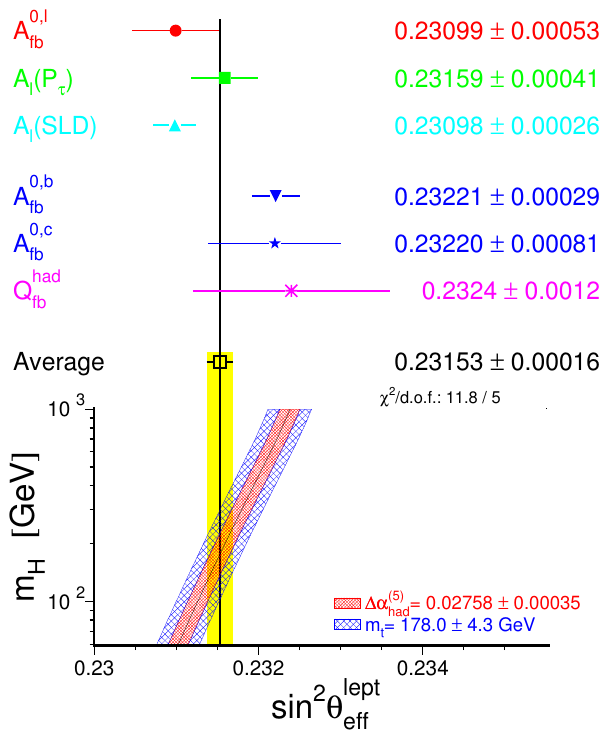
\includegraphics[width=0.5\linewidth]{elektroweak_precision_tests/h_massa_voorspelling.png}
    \caption{Voorspellingen voor de massa van het Higgs boson}%
    \label{fig:elektroweak_precision_tests/h_massa_voorspelling}
\end{figure}
Ondertussen hebben we $\theta_W$ al heel precies gemeten en weten we ook wat de massa van $t$ is. Zo kunnen we een range vinden wat de massa van het Higgs boson kan zijn. Dit wordt weergeven in figuur \ref{fig:elektroweak_precision_tests/h_massa_voorspelling} waarbij de Higgs massa kan liggen tussen $100$GeV en $300$GeV. Een 2de manier om deze voorspelling te bekomen is door de relatie tussen de massa van het $W$ boson en de massa van de $t$ quark te bekijken in figuur \ref{fig:elektroweak_precision_tests/h_massa_voorspelling_2}. Hier is terug duidelijk dat de massa van het Higgs boson verrassend klein moet zijn.

\begin{figure}[h]
    \centering
    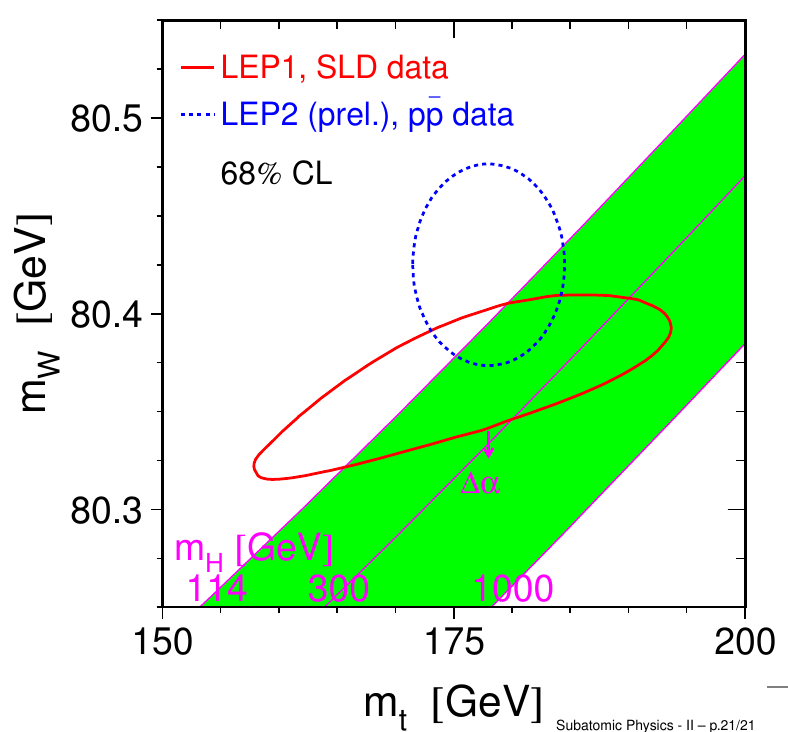
\includegraphics[width=0.4\linewidth]{elektroweak_precision_tests/h_massa_voorspelling_2.png}
    \caption{Voorspelling van de massa van het Higgs boson in meer detail}%
    \label{fig:elektroweak_precision_tests/h_massa_voorspelling_2}
\end{figure}

Het Higgs boson is niet gevonden tijdens de metingen in het LEP tot op $110$GeV. Hierdoor kunnen we het Higgs met een lagere massa dan $110$GeV uitsluiten. Waar we het Higgs boson zouden tegenkomen was dus eigenlijk heel goed voorspelt ($M_H = 129_{-49}^{+74}$GeV).

\end{document}
